\section{Discharge Apparatus}

The design of the discharge apparatus was similar to the coaxial geometry used
by Vasilyak and others \cite{Vasilyak1994}. This configuration has the benefit
of minimizing the inductance of the system, which should aid in the propagation
of the pulse through the system. Figure~\ref{fig:appschem}
\begin{figure}
  \centering
  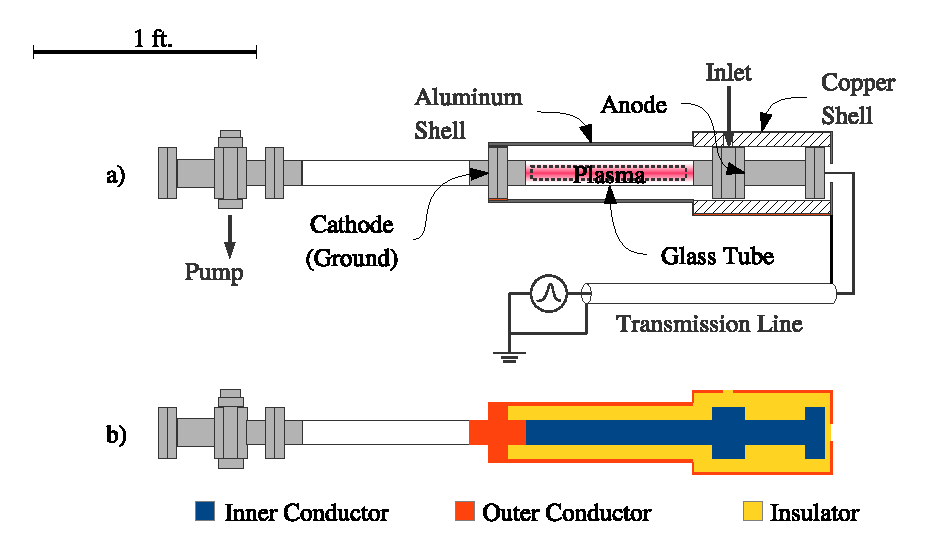
\includegraphics{./chapters/experiment/figures/appschem.eps}
  \caption{A scaled illustration of the discharge apparatus used in the
  \acs{rpnd} experiment.}
  \label{fig:appschem}
\end{figure}
is a to-scale illustration of the discharge apparatus.

The main portion of the discharge was provided by a borosilicate glass tube with
Conflat flanges on either end. The glass portion of the tube had an inner
diameter of 3.3 cm, an outer diameter of 4.0 cm, and a length of 22.9 cm. The
total length of tube, including the glass tube, glass-to-metal transition, and
flanges was 30 cm. The flanges served as the electrodes for the plasma. Seen
here, the anode is located on the right, and the cathode/ground is located on
the left.

The cathode was connected to a second glass tube with the same dimensions as the
first. This tube led to the pumping apparatus and served to electrically isolate
it from the rest of the system. The cathode was also connected to ground through
a cylindrical ground shell which ran along the outside of the discharge tube.
The ground shell was held in place against the cathode with a copper shim and
Delrin shaft collar.

Two slots were milled into the ground shell on opposite sides. The slots were
3.8 cm by 30 cm and served to provide optical access to the discharge tube. The
side of the ground shell opposite the cathode terminated at a copper sheet, 10
cm square. The copper sheet was perpendicular to the axis of the discharge tube
and had a 5 cm hole for discharge tube to pass through. The ground shell was
connected to the copper sheet with conductive copper tape.

The copper sheet was secured to a Teflon tube, approximately 20 cm in length
with an inner diameter of about 7.5 cm and an outer diameter of 10 cm. The
Teflon tube provided electrical isolation for the anode from structures
supporting it. Surrounding the Teflon tube was a second ground shell composed of
copper. This was connected to the first ground shell by a braided copper strap.
The other end of the second ground shell ended in a similar square copper sheet,
10 cm on each side. This sheet was secured to the Teflon tube by nylon screws
and seated against the ground shell for electrical contact.

The copper sheet also featured a HN bulkhead adapter for connection to the
transmission line. The inner conductor of the bulkhead adapter was connected by
a straight run of 5 cm of silicone-coated wire to a Conflat window angled at
45$^\cdot$. The window was connected to a Conflat nipple, which in turn was
connected to a double-sided flange used as the gas inlet (access was provided by
a 2.54 cm diameter hole drilled into the surrounding Teflon tube). The other
side of the double-sided flange was connected to the anode of the discharge
tube.

The voltage pulse was provided by a \acs{fid} pulser, supplied by \textsc{anvs},
Inc. (model \smaller{PT510NM}). The amplitude of the pulse was fixed at 6.6 kV
with a repetition rate of 1.0 kHz. It is likely that the low conductivity of the
gas preceding each pulse resulted in a doubling of the pulse potential as it
reflected from the electrode. A \textsc{srs} \smaller{DG645} delay generator was
used as the master clock in all experiments and was used to trigger the pulser.
A 13.7 m transmission line was used in order to isolate reflections traveling
back and forth between the pulser and anode. The cable used was RG213, and HN
connectors were used to prevent breakdown between the center conductor and
ground.

The gas inlet connection was made through the double-sided flange via a 1/8"
\textsc{npt} hole. A 1/4" polyethylene tube was attached to the \textsc{npt}
connection via a \textsc{npt} to 1/4" Swagelok adapater. The tube was then
connected by Swagelok to a source of ultra-high purity (99.999\%) helium.
Throughout the experiment, the helium flow rate was fixed at 25.0 sccm with a
digital flow controller, regardless of the operating pressure.

The discharge apparatus was pumped down by a oil-based roughing pump with an
upstream zeolite trap. In each case, the system was evacuated by the roughing
pump to the base pressure, approximately 15 mTorr, via a large-diameter tube.
Based on this, the level of background impurities was estimated to be 80 ppm.
This pump path was the closed off, and additional pumping was performed via two
needle valve bypasses. The needle valves were used to adjust the pump rate in
order to obtain the desired system pressure, monitored by two capacitance
manometers with ranges of 10 and 100 Torr.

The assembled discharge apparatus can be seen in figure~\ref{fig:appphoto}.
\begin{figure}
  \centering
  \setlength\fboxsep{0pt}
  \setlength\fboxrule{1.0pt}
  \fbox{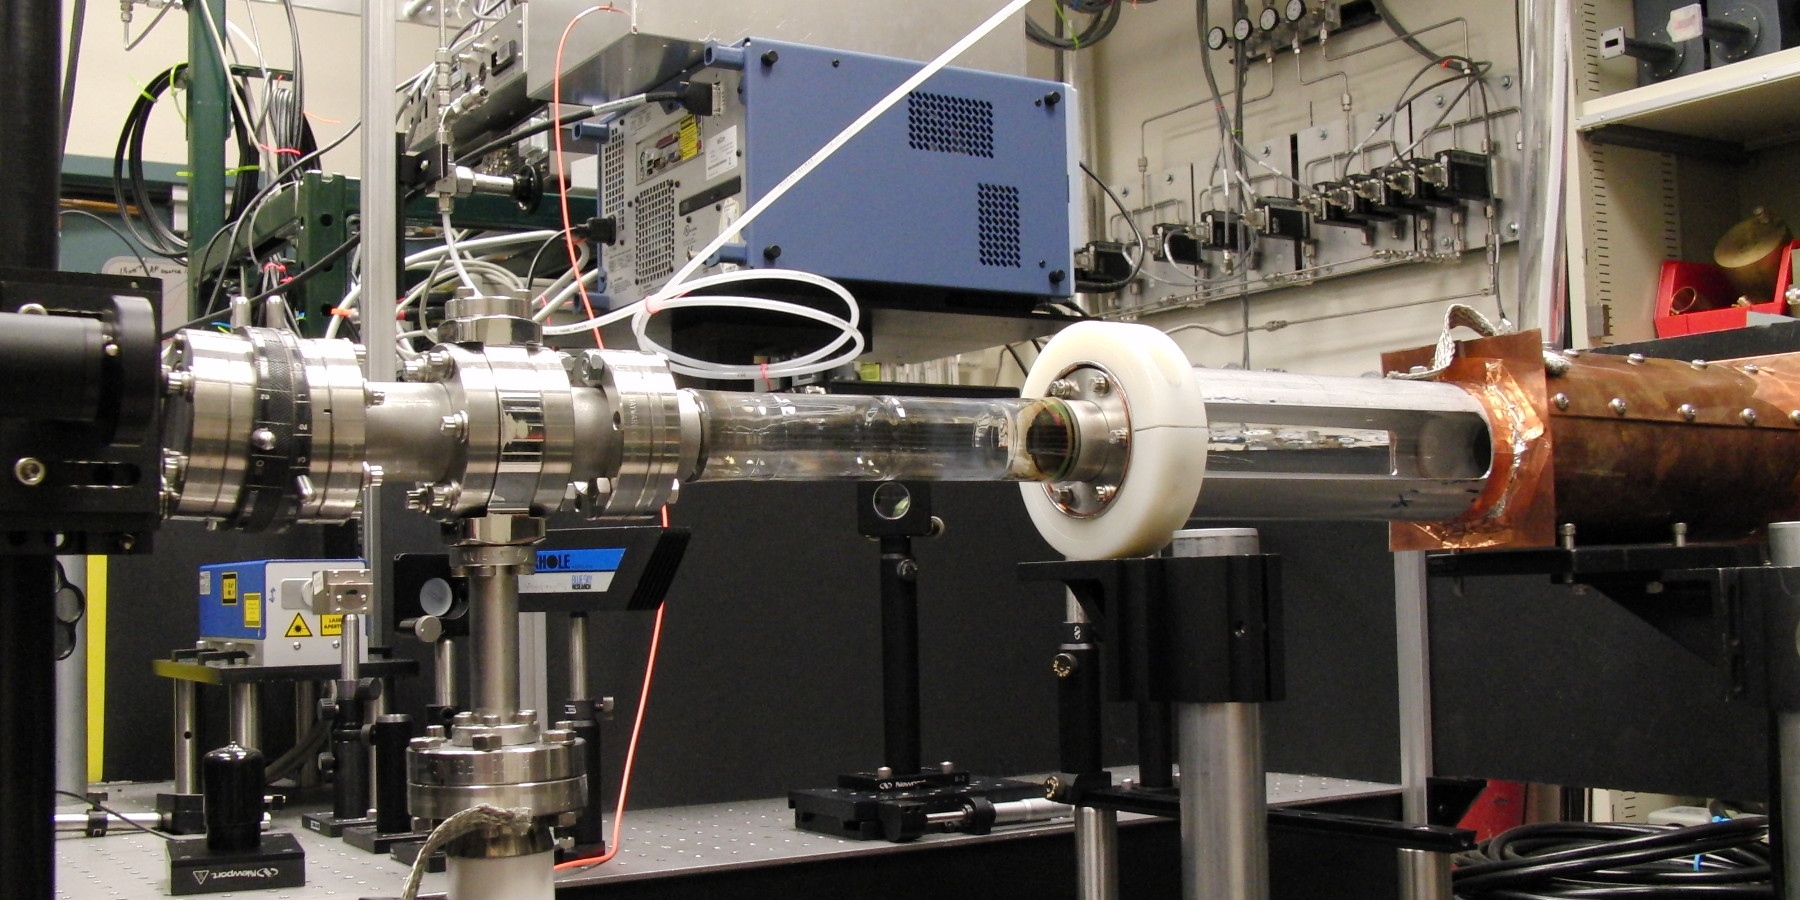
\includegraphics{./chapters/experiment/figures/appphoto.jpg}}
  \caption{Photograph of the discharge apparatus.}
  \label{fig:appphoto}
\end{figure}
The apparatus was supported on an optical breadboard 2.54 cm diameter posts and
angle brackets. Attached to one of the angle brackets was a small optical
breadboard with four bolts which served as physical references for aligning and
positioning the apparatus.

All electrical measurements were made with a LeCroy \smaller{6100A} WaveRunner
oscilloscope which had a bandwidth of 1.0 GHz. Electrical connections to the
oscilloscope were made with the shortest practical lengths of \smaller{RG 50/U}
coaxial cable and terminated at 50 $\Omega$ unless otherwise noted. The voltage
of the pulser was monitored from an internal $1:1000$ divider, and the current
was via a current shunt located in a break of the outer conductor of the
transmission line. The current shunt was composed of 9, low inductance, $1.0
\Omega$ resistors connected in parallel. Figure~\ref{fig:bcs}
\begin{figure}
  \centering
  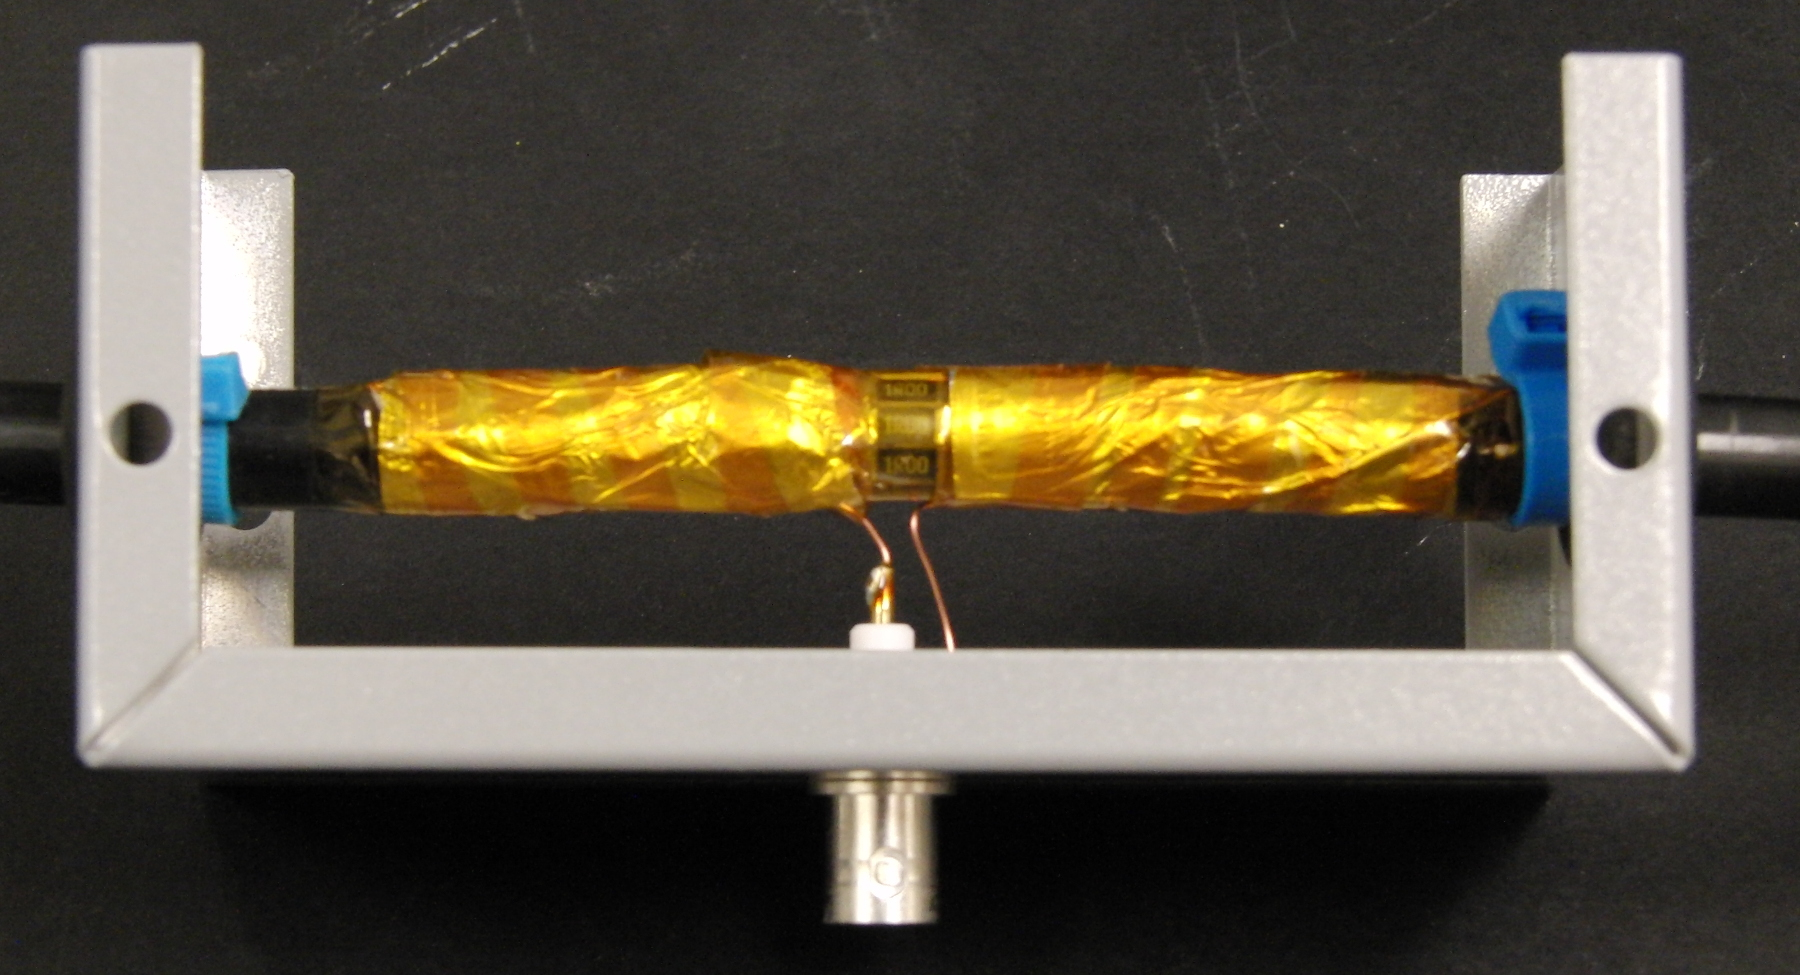
\includegraphics{./chapters/experiment/figures/bcs.jpg}
  \caption{Photograph of the back-current shunt used to measure the current
  characteristics of the \acs{rpnd}.}
  \label{fig:bcs}
\end{figure}

Data were retrieved from the oscilloscope with a desktop computer via a
\textsc{gpib} connection. A LabView interface was used to interface with the
oscilloscope and additional instruments. Analog inputs and outputs (such as
laser control and pressure sensing) were handled by a \textsc{srs}
\smaller{sr850 dsp} lock-in amplifier which performed as an \emph{ad hoc} data
acquisition system.

\section{Operating Procedure \& Conditions}

At the beginning of each day of operation, the system was first pumped down to
base pressure. After this, the primary pump path was closed in favor of the
needle valve bypasses. The helium flow was then initiated at 25.0 sccm. Then,
the system pressure was adjusted to 3.0 Torr.

Once the pressure reached equilibrium, the pulser was turned on. The plasma was
allowed to run at this condition for one hour in order to remove built up
contamination on the walls and electrodes. During this time, the pressure of the
system would typically drift downwards by several percent. Afterward, the
pressure would be adjusted to the desired operating condition.

It was frequently necessary to turn off the pulser in between experiments. In
these cases, once the pulser was turned on, the plasma was allowed to run for 15
minutes before any measurements were made. This was necessitated by observable
changes in the emissions and current-voltage characteristics during the first 15
minutes of operation. Additional increases to this warm up time resulted in no
appreciable changes to any of the measured data.

Measurements were made for a range of pressures, including: 0.3, 0.5, 1.0, 2.0
3.0, 4.0, 8.0, and 16.0 Torr. The lower limit was set by the pumping speed of
the roughing pump. Difficulty in obtaining reliable plasma breakdown at
pressures above 16.0 Torr set an upper limit on the pressure range. Experimental
measurements of optical properties were obtained at three axial locations: 7.6,
15.2, and 22.9 cm, relative to the anode. These will frequently be referred to
as upstream, midstream, and downstream locations, respectively.

\section{Initial Observations}


\section{Energy Coupling}


\section{Absorption Setup}
The \acs{las} setup was based upon the used of a distributed-feedback
laser diode. Temperature and current control of the diode provided
coarse and fine tuning, respectively, for the output frequency. It was
found that it was unnecessary to adjust the temperature for the diode
once the correct transition was found, therefore all tuning was
accomplished using current tuning.

The laser diode was produced by Toptica Photonics (model
\#LD-1083-0070-DFB-1), and had a nominal operating power of 70 mW at a
center wavelength of 1083 nm. The diode was held inside a Toptica DL-100
diode housing which contained an integral thermoelectric cooler and
collimating optics. The operation of the diode was controlled by a
Toptica DC 110 monitor, DCC 110 current control, DTC 110 temperature
control, and SC 110 scan control.

A schematic of the optical layout for the absorption experiment can be
seen in Figure \ref{fig:abslayout}. Immediately after exiting the
housing, the beam was passed through an optical isolator in order to
prevent instabilities from back reflections. Next the beam was
attenuated using a neutral density filter in order to keep its intensity
below the saturation level for the transition. Following that, the beam
passed through two apertures for alignment. Here, the beam was split by
a partially reflecting mirror. Approximately 98\% of the beam was
allowed to pass through to a reference photodiode (Thorlabs DET300).
After passing through the plasma, entered another aperture to limit
near-coincident plasma emissions. The background emissions were further
reduced using a long pass filter with a cutoff of 1000 nm. Finally, the
beam was coupled into an optical fiber which connected to the detection
electronics.

The transmitted laser light was detected with an InGaAs photodiode
(Thorlabs DET410). The signal from the diode was often too small to
detect, so the output of the signal photodiode was sent through a
voltage amplifier (Femto HVA-200M-40-B). The light response of this
system is limited by the photodiode which has a nominal rise time of
five nanoseconds. The signal from the amplifier was terminated by a 50
ohm terminator and sensed by the aforementioned oscilloscope.

\subsection{Acquisition Process} The actual acquisition process required
a specific series of steps in order to properly account for all noise
sources. In order to accommodate this process, a custom LabView script
was used to automate the acquisition of the laser transmission spectra.
Generally speaking, the signal can be described as
\begin{equation}
  V_\mathrm{total} = V_\mathrm{signal} + V_\mathrm{background} +
                     V_\mathrm{plasma}.
\end{equation}
In order to remove the background signal, the acquisition scr

\section{Emissions Setup}
